\documentclass{standalone}
\usepackage{tikz}
\usetikzlibrary{patterns, positioning}

\begin{document}
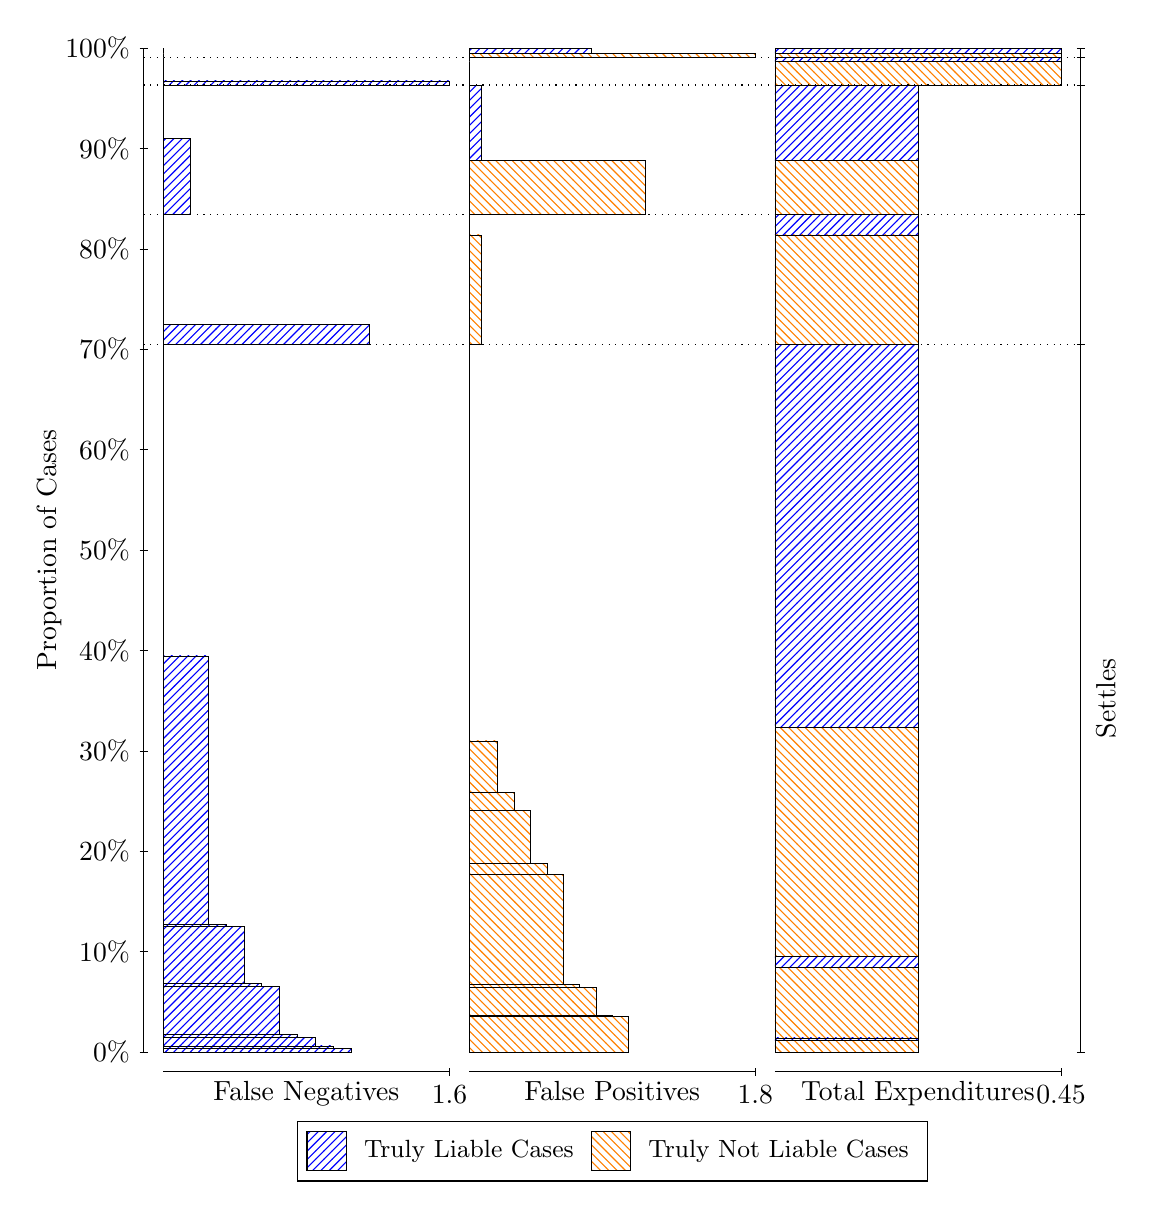
\begin{tikzpicture}
\draw[black, very thin] (1.5,1.75) -- (1.5,14.5);
\node[rotate=90, anchor=center] at (0.3, 8.125) {Proportion of Cases};
\draw[black, very thin] (1.45,1.75) -- (1.55,1.75);
\node[anchor=east] at (1.45, 1.75) {0\%};
\draw[black, very thin] (1.45,3.025) -- (1.55,3.025);
\node[anchor=east] at (1.45, 3.025) {10\%};
\draw[black, very thin] (1.45,4.3) -- (1.55,4.3);
\node[anchor=east] at (1.45, 4.3) {20\%};
\draw[black, very thin] (1.45,5.575) -- (1.55,5.575);
\node[anchor=east] at (1.45, 5.575) {30\%};
\draw[black, very thin] (1.45,6.85) -- (1.55,6.85);
\node[anchor=east] at (1.45, 6.85) {40\%};
\draw[black, very thin] (1.45,8.125) -- (1.55,8.125);
\node[anchor=east] at (1.45, 8.125) {50\%};
\draw[black, very thin] (1.45,9.4) -- (1.55,9.4);
\node[anchor=east] at (1.45, 9.4) {60\%};
\draw[black, very thin] (1.45,10.675) -- (1.55,10.675);
\node[anchor=east] at (1.45, 10.675) {70\%};
\draw[black, very thin] (1.45,11.95) -- (1.55,11.95);
\node[anchor=east] at (1.45, 11.95) {80\%};
\draw[black, very thin] (1.45,13.225) -- (1.55,13.225);
\node[anchor=east] at (1.45, 13.225) {90\%};
\draw[black, very thin] (1.45,14.5) -- (1.55,14.5);
\node[anchor=east] at (1.45, 14.5) {100\%};

\draw[black, very thin] (13.4,1.75) -- (13.4,14.5);
\draw[black, very thin] (13.35,1.75) -- (13.45,1.75);
\node[anchor=west] at (13.35, 1.75) {};
\draw[black, very thin] (13.35,10.733) -- (13.45,10.733);
\node[anchor=west] at (13.35, 10.733) {};
\draw[black, very thin] (13.35,12.388) -- (13.45,12.388);
\node[anchor=west] at (13.35, 12.388) {};
\draw[black, very thin] (13.35,14.03) -- (13.45,14.03);
\node[anchor=west] at (13.35, 14.03) {};
\draw[black, very thin] (13.35,14.379) -- (13.45,14.379);
\node[anchor=west] at (13.35, 14.379) {};
\draw[black, very thin] (13.35,14.5) -- (13.45,14.5);
\node[anchor=west] at (13.35, 14.5) {};

\draw[black, very thin, pattern color=blue, pattern=north east lines] (1.75,1.75) rectangle (4.1344,1.8004);
\draw[black, very thin, pattern color=blue, pattern=north east lines] (1.75,1.8004) rectangle (3.9073,1.827);
\draw[black, very thin, pattern color=blue, pattern=north east lines] (1.75,1.827) rectangle (3.6802,1.9373);
\draw[black, very thin, pattern color=blue, pattern=north east lines] (1.75,1.9373) rectangle (3.4531,1.9732);
\draw[black, very thin, pattern color=blue, pattern=north east lines] (1.75,1.9732) rectangle (3.226,2.5832);
\draw[black, very thin, pattern color=blue, pattern=north east lines] (1.75,2.5832) rectangle (2.999,2.6197);
\draw[black, very thin, pattern color=blue, pattern=north east lines] (1.75,2.6197) rectangle (2.7719,3.3446);
\draw[black, very thin, pattern color=blue, pattern=north east lines] (1.75,3.3446) rectangle (2.5448,3.3687);
\draw[black, very thin, pattern color=blue, pattern=north east lines] (1.75,3.3687) rectangle (2.3177,6.7816);
\draw[black, very thin, pattern color=orange, pattern=north west lines] (1.75,6.7816) rectangle (1.75,10.733);
\draw[black, very thin, pattern color=blue, pattern=north east lines] (1.75,10.733) rectangle (4.3615,10.995);
\draw[black, very thin, pattern color=orange, pattern=north west lines] (1.75,10.995) rectangle (1.75,12.388);
\draw[black, very thin, pattern color=blue, pattern=north east lines] (1.75,12.388) rectangle (2.0906,13.348);
\draw[black, very thin, pattern color=orange, pattern=north west lines] (1.75,13.348) rectangle (1.75,14.03);
\draw[black, very thin, pattern color=blue, pattern=north east lines] (1.75,14.03) rectangle (5.3833,14.083);
\draw[black, very thin, pattern color=orange, pattern=north west lines] (1.75,14.083) rectangle (1.75,14.379);
\draw[black, very thin, pattern color=orange, pattern=north west lines] (1.75,14.379) rectangle (1.75,14.431);
\draw[black, very thin, pattern color=blue, pattern=north east lines] (1.75,14.431) rectangle (1.75,14.5);
\draw[black, very thin, pattern color=orange, pattern=north west lines] (5.6333,1.75) rectangle (7.6576,2.1989);
\draw[black, very thin, pattern color=orange, pattern=north west lines] (5.6333,2.1989) rectangle (7.45,2.2136);
\draw[black, very thin, pattern color=orange, pattern=north west lines] (5.6333,2.2136) rectangle (7.2424,2.5723);
\draw[black, very thin, pattern color=orange, pattern=north west lines] (5.6333,2.5723) rectangle (7.0348,2.6077);
\draw[black, very thin, pattern color=orange, pattern=north west lines] (5.6333,2.6077) rectangle (6.8271,4.001);
\draw[black, very thin, pattern color=orange, pattern=north west lines] (5.6333,4.001) rectangle (6.6195,4.1445);
\draw[black, very thin, pattern color=orange, pattern=north west lines] (5.6333,4.1445) rectangle (6.6195,4.1492);
\draw[black, very thin, pattern color=orange, pattern=north west lines] (5.6333,4.1492) rectangle (6.4119,4.8201);
\draw[black, very thin, pattern color=orange, pattern=north west lines] (5.6333,4.8201) rectangle (6.2043,5.0441);
\draw[black, very thin, pattern color=orange, pattern=north west lines] (5.6333,5.0441) rectangle (5.9967,5.7017);
\draw[black, very thin, pattern color=blue, pattern=north east lines] (5.6333,5.7017) rectangle (5.6333,10.733);
\draw[black, very thin, pattern color=orange, pattern=north west lines] (5.6333,10.733) rectangle (5.789,12.127);
\draw[black, very thin, pattern color=blue, pattern=north east lines] (5.6333,12.127) rectangle (5.6333,12.388);
\draw[black, very thin, pattern color=orange, pattern=north west lines] (5.6333,12.388) rectangle (7.8652,13.071);
\draw[black, very thin, pattern color=blue, pattern=north east lines] (5.6333,13.071) rectangle (5.789,14.03);
\draw[black, very thin, pattern color=orange, pattern=north west lines] (5.6333,14.03) rectangle (5.6333,14.326);
\draw[black, very thin, pattern color=blue, pattern=north east lines] (5.6333,14.326) rectangle (5.6333,14.379);
\draw[black, very thin, pattern color=orange, pattern=north west lines] (5.6333,14.379) rectangle (9.2667,14.431);
\draw[black, very thin, pattern color=blue, pattern=north east lines] (5.6333,14.431) rectangle (7.1905,14.5);
\draw[black, very thin, pattern color=orange, pattern=north west lines] (9.5167,1.75) rectangle (11.333,1.8935);
\draw[black, very thin, pattern color=blue, pattern=north east lines] (9.5167,1.8935) rectangle (11.333,1.9283);
\draw[black, very thin, pattern color=orange, pattern=north west lines] (9.5167,1.9283) rectangle (11.333,2.8279);
\draw[black, very thin, pattern color=blue, pattern=north east lines] (9.5167,2.8279) rectangle (11.333,2.9659);
\draw[black, very thin, pattern color=orange, pattern=north west lines] (9.5167,2.9659) rectangle (11.333,5.8745);
\draw[black, very thin, pattern color=blue, pattern=north east lines] (9.5167,5.8745) rectangle (11.333,10.733);
\draw[black, very thin, pattern color=orange, pattern=north west lines] (9.5167,10.733) rectangle (11.333,12.127);
\draw[black, very thin, pattern color=blue, pattern=north east lines] (9.5167,12.127) rectangle (11.333,12.388);
\draw[black, very thin, pattern color=orange, pattern=north west lines] (9.5167,12.388) rectangle (11.333,13.071);
\draw[black, very thin, pattern color=blue, pattern=north east lines] (9.5167,13.071) rectangle (11.333,14.03);
\draw[black, very thin, pattern color=orange, pattern=north west lines] (9.5167,14.03) rectangle (13.15,14.326);
\draw[black, very thin, pattern color=blue, pattern=north east lines] (9.5167,14.326) rectangle (13.15,14.379);
\draw[black, very thin, pattern color=orange, pattern=north west lines] (9.5167,14.379) rectangle (13.15,14.431);
\draw[black, very thin, pattern color=blue, pattern=north east lines] (9.5167,14.431) rectangle (13.15,14.5);
\draw[black, dotted] (1.5,10.733) -- (13.4,10.733);
\draw[black, dotted] (1.5,12.388) -- (13.4,12.388);
\draw[black, dotted] (1.5,14.03) -- (13.4,14.03);
\draw[black, dotted] (1.5,14.379) -- (13.4,14.379);
\draw[black, very thin] (1.75,1.5) -- (5.3833,1.5);
\node[anchor=north] at (3.5667, 1.5) {False Negatives};
\draw[black, very thin] (5.3833,1.45) -- (5.3833,1.55);
\node[anchor=north] at (5.3833, 1.45) {1.6};

\draw[black, very thin] (5.6333,1.5) -- (9.2667,1.5);
\node[anchor=north] at (7.45, 1.5) {False Positives};
\draw[black, very thin] (9.2667,1.45) -- (9.2667,1.55);
\node[anchor=north] at (9.2667, 1.45) {1.8};

\draw[black, very thin] (9.5167,1.5) -- (13.15,1.5);
\node[anchor=north] at (11.333, 1.5) {Total Expenditures};
\draw[black, very thin] (13.15,1.45) -- (13.15,1.55);
\node[anchor=north] at (13.15, 1.45) {0.45};

\node[black, centered, rotate=90] at (13.72, 6.2417) {Settles};





\draw (7.449999999999999,1.5) node[draw=none] (baseCoordinate) {};
\begin{scope}[align=center]
        \matrix[scale=0.5, draw=black, below=0.5cm of baseCoordinate, nodes={draw}, column sep=0.1cm]{
            \node[rectangle, draw, minimum width=0.5cm, minimum height=0.5cm, pattern=north east lines, pattern color=blue] {}; &
            \node[draw=none, font=\small] (B) {Truly Liable Cases}; &
            \node[rectangle, draw, minimum width=0.5cm, minimum height=0.5cm, pattern=north west lines, pattern color=orange] {}; &
            \node[draw=none, font=\small] (B) {Truly Not Liable Cases}; \\
            };
\end{scope}

\end{tikzpicture}
\end{document}